% Options for packages loaded elsewhere
\PassOptionsToPackage{unicode}{hyperref}
\PassOptionsToPackage{hyphens}{url}
%
\documentclass[
]{article}
\usepackage{lmodern}
\usepackage{amssymb,amsmath}
\usepackage{ifxetex,ifluatex}
\ifnum 0\ifxetex 1\fi\ifluatex 1\fi=0 % if pdftex
  \usepackage[T1]{fontenc}
  \usepackage[utf8]{inputenc}
  \usepackage{textcomp} % provide euro and other symbols
\else % if luatex or xetex
  \usepackage{unicode-math}
  \defaultfontfeatures{Scale=MatchLowercase}
  \defaultfontfeatures[\rmfamily]{Ligatures=TeX,Scale=1}
\fi
% Use upquote if available, for straight quotes in verbatim environments
\IfFileExists{upquote.sty}{\usepackage{upquote}}{}
\IfFileExists{microtype.sty}{% use microtype if available
  \usepackage[]{microtype}
  \UseMicrotypeSet[protrusion]{basicmath} % disable protrusion for tt fonts
}{}
\makeatletter
\@ifundefined{KOMAClassName}{% if non-KOMA class
  \IfFileExists{parskip.sty}{%
    \usepackage{parskip}
  }{% else
    \setlength{\parindent}{0pt}
    \setlength{\parskip}{6pt plus 2pt minus 1pt}}
}{% if KOMA class
  \KOMAoptions{parskip=half}}
\makeatother
\usepackage{xcolor}
\IfFileExists{xurl.sty}{\usepackage{xurl}}{} % add URL line breaks if available
\IfFileExists{bookmark.sty}{\usepackage{bookmark}}{\usepackage{hyperref}}
\hypersetup{
  pdftitle={COAP: simulation},
  pdfauthor={Wei Liu},
  hidelinks,
  pdfcreator={LaTeX via pandoc}}
\urlstyle{same} % disable monospaced font for URLs
\usepackage[margin=1in]{geometry}
\usepackage{color}
\usepackage{fancyvrb}
\newcommand{\VerbBar}{|}
\newcommand{\VERB}{\Verb[commandchars=\\\{\}]}
\DefineVerbatimEnvironment{Highlighting}{Verbatim}{commandchars=\\\{\}}
% Add ',fontsize=\small' for more characters per line
\usepackage{framed}
\definecolor{shadecolor}{RGB}{248,248,248}
\newenvironment{Shaded}{\begin{snugshade}}{\end{snugshade}}
\newcommand{\AlertTok}[1]{\textcolor[rgb]{0.94,0.16,0.16}{#1}}
\newcommand{\AnnotationTok}[1]{\textcolor[rgb]{0.56,0.35,0.01}{\textbf{\textit{#1}}}}
\newcommand{\AttributeTok}[1]{\textcolor[rgb]{0.77,0.63,0.00}{#1}}
\newcommand{\BaseNTok}[1]{\textcolor[rgb]{0.00,0.00,0.81}{#1}}
\newcommand{\BuiltInTok}[1]{#1}
\newcommand{\CharTok}[1]{\textcolor[rgb]{0.31,0.60,0.02}{#1}}
\newcommand{\CommentTok}[1]{\textcolor[rgb]{0.56,0.35,0.01}{\textit{#1}}}
\newcommand{\CommentVarTok}[1]{\textcolor[rgb]{0.56,0.35,0.01}{\textbf{\textit{#1}}}}
\newcommand{\ConstantTok}[1]{\textcolor[rgb]{0.00,0.00,0.00}{#1}}
\newcommand{\ControlFlowTok}[1]{\textcolor[rgb]{0.13,0.29,0.53}{\textbf{#1}}}
\newcommand{\DataTypeTok}[1]{\textcolor[rgb]{0.13,0.29,0.53}{#1}}
\newcommand{\DecValTok}[1]{\textcolor[rgb]{0.00,0.00,0.81}{#1}}
\newcommand{\DocumentationTok}[1]{\textcolor[rgb]{0.56,0.35,0.01}{\textbf{\textit{#1}}}}
\newcommand{\ErrorTok}[1]{\textcolor[rgb]{0.64,0.00,0.00}{\textbf{#1}}}
\newcommand{\ExtensionTok}[1]{#1}
\newcommand{\FloatTok}[1]{\textcolor[rgb]{0.00,0.00,0.81}{#1}}
\newcommand{\FunctionTok}[1]{\textcolor[rgb]{0.00,0.00,0.00}{#1}}
\newcommand{\ImportTok}[1]{#1}
\newcommand{\InformationTok}[1]{\textcolor[rgb]{0.56,0.35,0.01}{\textbf{\textit{#1}}}}
\newcommand{\KeywordTok}[1]{\textcolor[rgb]{0.13,0.29,0.53}{\textbf{#1}}}
\newcommand{\NormalTok}[1]{#1}
\newcommand{\OperatorTok}[1]{\textcolor[rgb]{0.81,0.36,0.00}{\textbf{#1}}}
\newcommand{\OtherTok}[1]{\textcolor[rgb]{0.56,0.35,0.01}{#1}}
\newcommand{\PreprocessorTok}[1]{\textcolor[rgb]{0.56,0.35,0.01}{\textit{#1}}}
\newcommand{\RegionMarkerTok}[1]{#1}
\newcommand{\SpecialCharTok}[1]{\textcolor[rgb]{0.00,0.00,0.00}{#1}}
\newcommand{\SpecialStringTok}[1]{\textcolor[rgb]{0.31,0.60,0.02}{#1}}
\newcommand{\StringTok}[1]{\textcolor[rgb]{0.31,0.60,0.02}{#1}}
\newcommand{\VariableTok}[1]{\textcolor[rgb]{0.00,0.00,0.00}{#1}}
\newcommand{\VerbatimStringTok}[1]{\textcolor[rgb]{0.31,0.60,0.02}{#1}}
\newcommand{\WarningTok}[1]{\textcolor[rgb]{0.56,0.35,0.01}{\textbf{\textit{#1}}}}
\usepackage{graphicx,grffile}
\makeatletter
\def\maxwidth{\ifdim\Gin@nat@width>\linewidth\linewidth\else\Gin@nat@width\fi}
\def\maxheight{\ifdim\Gin@nat@height>\textheight\textheight\else\Gin@nat@height\fi}
\makeatother
% Scale images if necessary, so that they will not overflow the page
% margins by default, and it is still possible to overwrite the defaults
% using explicit options in \includegraphics[width, height, ...]{}
\setkeys{Gin}{width=\maxwidth,height=\maxheight,keepaspectratio}
% Set default figure placement to htbp
\makeatletter
\def\fps@figure{htbp}
\makeatother
\setlength{\emergencystretch}{3em} % prevent overfull lines
\providecommand{\tightlist}{%
  \setlength{\itemsep}{0pt}\setlength{\parskip}{0pt}}
\setcounter{secnumdepth}{-\maxdimen} % remove section numbering

\title{COAP: simulation}
\author{Wei Liu}
\date{2023-08-12}

\begin{document}
\maketitle

This vignette introduces the usage of COAP for the analysis of
high-dimensional count data with additional high-dimensional covariates,
by comparison with other methods.

The package can be loaded with the command:

\begin{Shaded}
\begin{Highlighting}[]
\KeywordTok{library}\NormalTok{(COAP)}
\KeywordTok{library}\NormalTok{(GFM)}
\end{Highlighting}
\end{Shaded}

\hypertarget{generate-the-simulated-data}{%
\subsection{Generate the simulated
data}\label{generate-the-simulated-data}}

First, we generate the data simulated data.

\begin{Shaded}
\begin{Highlighting}[]
\KeywordTok{set.seed}\NormalTok{(}\DecValTok{1}\NormalTok{)}
\NormalTok{n <-}\StringTok{ }\DecValTok{200}\NormalTok{; p <-}\StringTok{ }\DecValTok{200}\NormalTok{; }
\NormalTok{d=}\StringTok{ }\DecValTok{50}
\NormalTok{rank0 <-}\StringTok{ }\DecValTok{6}\NormalTok{;}
\NormalTok{q =}\StringTok{ }\DecValTok{5}\NormalTok{;}
\NormalTok{datList <-}\StringTok{ }\KeywordTok{gendata_simu}\NormalTok{(}\DataTypeTok{seed =} \DecValTok{1}\NormalTok{, }\DataTypeTok{n=}\NormalTok{n, }\DataTypeTok{p=}\NormalTok{p, }\DataTypeTok{d=}\NormalTok{ d, }\DataTypeTok{rank0 =}\NormalTok{ rank0, }\DataTypeTok{q=}\NormalTok{ q, }\DataTypeTok{rho=}\KeywordTok{c}\NormalTok{(}\DecValTok{2}\NormalTok{, }\DecValTok{2}\NormalTok{),}
                        \DataTypeTok{sigma2_eps =} \DecValTok{1}\NormalTok{)}
\NormalTok{X_count <-}\StringTok{ }\NormalTok{datList}\OperatorTok{$}\NormalTok{X; Z <-}\StringTok{ }\NormalTok{datList}\OperatorTok{$}\NormalTok{Z}
\NormalTok{H0 <-}\StringTok{ }\NormalTok{datList}\OperatorTok{$}\NormalTok{H0; B0 <-}\StringTok{ }\NormalTok{datList}\OperatorTok{$}\NormalTok{B0}
\NormalTok{bbeta0 <-}\StringTok{ }\KeywordTok{cbind}\NormalTok{( datList}\OperatorTok{$}\NormalTok{mu0, datList}\OperatorTok{$}\NormalTok{bbeta0)}
\end{Highlighting}
\end{Shaded}

Fit the COAP model using the function \texttt{RR\_COAP()} in the R
package \texttt{COAP}. Users can use \texttt{?RR\_COAP} to see the
details about this function

\begin{Shaded}
\begin{Highlighting}[]
\NormalTok{hq <-}\StringTok{ }\DecValTok{5}\NormalTok{; hr <-}\StringTok{ }\DecValTok{6}

\NormalTok{tic <-}\StringTok{ }\KeywordTok{proc.time}\NormalTok{()}
\NormalTok{reslist <-}\StringTok{ }\KeywordTok{RR_COAP}\NormalTok{(X_count, }\DataTypeTok{Z=}\NormalTok{ Z, }\DataTypeTok{q=}\NormalTok{hq, }\DataTypeTok{rank_use=}\NormalTok{ hr, }\DataTypeTok{epsELBO =} \FloatTok{1e-6}\NormalTok{)}
\CommentTok{#> Calculate initial values...}
\CommentTok{#> iter = 2, ELBO= 311531.420000, dELBO=1.000145 }
\CommentTok{#> iter = 3, ELBO= 316042.737970, dELBO=0.014481 }
\CommentTok{#> iter = 4, ELBO= 317869.490388, dELBO=0.005780 }
\CommentTok{#> iter = 5, ELBO= 318776.120476, dELBO=0.002852 }
\CommentTok{#> iter = 6, ELBO= 319290.972752, dELBO=0.001615 }
\CommentTok{#> iter = 7, ELBO= 319611.373938, dELBO=0.001003 }
\CommentTok{#> iter = 8, ELBO= 319824.015899, dELBO=0.000665 }
\CommentTok{#> iter = 9, ELBO= 319971.850666, dELBO=0.000462 }
\CommentTok{#> iter = 10, ELBO= 320078.245025, dELBO=0.000333 }
\CommentTok{#> iter = 11, ELBO= 320156.887531, dELBO=0.000246 }
\CommentTok{#> iter = 12, ELBO= 320216.278565, dELBO=0.000186 }
\CommentTok{#> iter = 13, ELBO= 320261.942528, dELBO=0.000143 }
\CommentTok{#> iter = 14, ELBO= 320297.599344, dELBO=0.000111 }
\CommentTok{#> iter = 15, ELBO= 320325.824786, dELBO=0.000088 }
\CommentTok{#> iter = 16, ELBO= 320348.442910, dELBO=0.000071 }
\CommentTok{#> iter = 17, ELBO= 320366.769724, dELBO=0.000057 }
\CommentTok{#> iter = 18, ELBO= 320381.769961, dELBO=0.000047 }
\CommentTok{#> iter = 19, ELBO= 320394.160880, dELBO=0.000039 }
\CommentTok{#> iter = 20, ELBO= 320404.482598, dELBO=0.000032 }
\CommentTok{#> iter = 21, ELBO= 320413.146652, dELBO=0.000027 }
\CommentTok{#> iter = 22, ELBO= 320420.470080, dELBO=0.000023 }
\CommentTok{#> iter = 23, ELBO= 320426.699664, dELBO=0.000019 }
\CommentTok{#> iter = 24, ELBO= 320432.029390, dELBO=0.000017 }
\CommentTok{#> iter = 25, ELBO= 320436.613167, dELBO=0.000014 }
\CommentTok{#> iter = 26, ELBO= 320440.574186, dELBO=0.000012 }
\CommentTok{#> iter = 27, ELBO= 320444.011876, dELBO=0.000011 }
\CommentTok{#> iter = 28, ELBO= 320447.007121, dELBO=0.000009 }
\CommentTok{#> iter = 29, ELBO= 320449.626207, dELBO=0.000008 }
\CommentTok{#> iter = 30, ELBO= 320451.923844, dELBO=0.000007}
\NormalTok{toc <-}\StringTok{ }\KeywordTok{proc.time}\NormalTok{()}
\NormalTok{time_coap <-}\StringTok{ }\NormalTok{toc[}\DecValTok{3}\NormalTok{] }\OperatorTok{-}\StringTok{ }\NormalTok{tic[}\DecValTok{3}\NormalTok{]}
\KeywordTok{message}\NormalTok{(time_coap, }\StringTok{" seconds"}\NormalTok{)}
\CommentTok{#> 0.670000000000073 seconds}
\end{Highlighting}
\end{Shaded}

Check the increased property of the envidence lower bound function.

\begin{Shaded}
\begin{Highlighting}[]
\KeywordTok{library}\NormalTok{(ggplot2)}
\NormalTok{dat_iter <-}\StringTok{ }\KeywordTok{data.frame}\NormalTok{(}\DataTypeTok{iter=}\DecValTok{1}\OperatorTok{:}\KeywordTok{length}\NormalTok{(reslist}\OperatorTok{$}\NormalTok{ELBO_seq), }\DataTypeTok{ELBO=}\NormalTok{reslist}\OperatorTok{$}\NormalTok{ELBO_seq)}
\KeywordTok{ggplot}\NormalTok{(}\DataTypeTok{data=}\NormalTok{dat_iter, }\KeywordTok{aes}\NormalTok{(}\DataTypeTok{x=}\NormalTok{iter, }\DataTypeTok{y=}\NormalTok{ELBO)) }\OperatorTok{+}\StringTok{ }\KeywordTok{geom_line}\NormalTok{() }\OperatorTok{+}\StringTok{ }\KeywordTok{geom_point}\NormalTok{() }\OperatorTok{+}\StringTok{ }\KeywordTok{theme_bw}\NormalTok{(}\DataTypeTok{base_size =} \DecValTok{20}\NormalTok{)}
\end{Highlighting}
\end{Shaded}

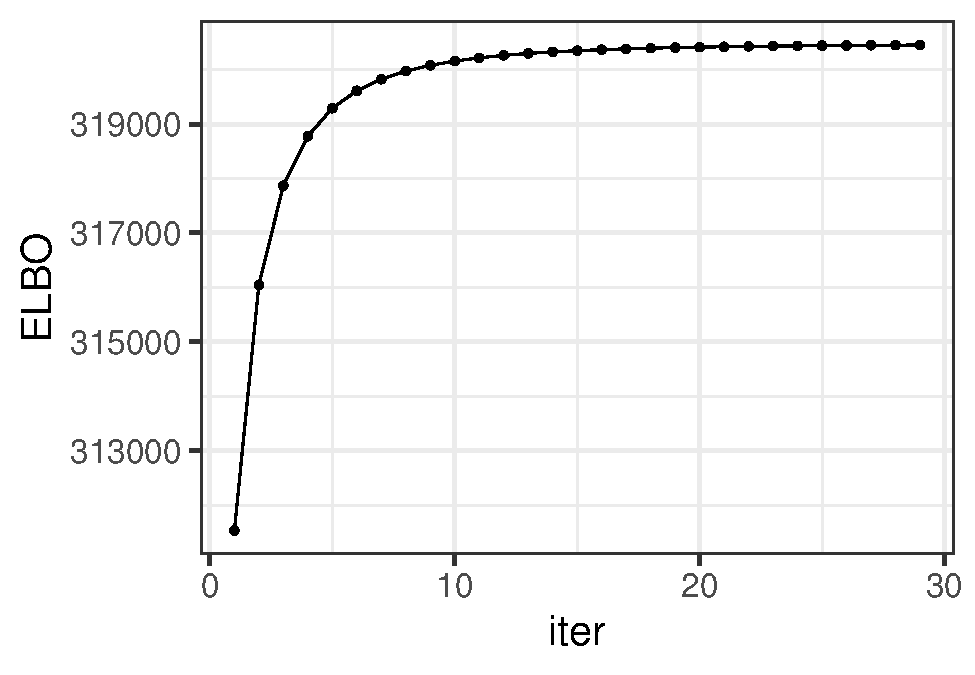
\includegraphics{COAPsimu_files/figure-latex/unnamed-chunk-5-1.pdf}

We calculate the metrics to measure the estimatioin accuracy, where the
trace statistic is used to measure the estimation accuracy of loading
matrix and prediction accuracy of factor matrix, which is evaluated by
the function \texttt{measurefun()} in the R package \texttt{GFM}, and
the root of mean square error is adopted to measure the estimation error
of bbeta.

\begin{Shaded}
\begin{Highlighting}[]
\KeywordTok{library}\NormalTok{(GFM)}
\NormalTok{metricList <-}\StringTok{ }\KeywordTok{list}\NormalTok{()}
\NormalTok{metricList}\OperatorTok{$}\NormalTok{COAP <-}\StringTok{ }\KeywordTok{list}\NormalTok{()}
\NormalTok{metricList}\OperatorTok{$}\NormalTok{COAP}\OperatorTok{$}\NormalTok{Tr_H <-}\StringTok{ }\KeywordTok{measurefun}\NormalTok{(reslist}\OperatorTok{$}\NormalTok{H, H0)}
\NormalTok{metricList}\OperatorTok{$}\NormalTok{COAP}\OperatorTok{$}\NormalTok{Tr_B <-}\StringTok{ }\KeywordTok{measurefun}\NormalTok{(reslist}\OperatorTok{$}\NormalTok{B, B0)}

\NormalTok{norm_vec <-}\StringTok{ }\ControlFlowTok{function}\NormalTok{(x) }\KeywordTok{sqrt}\NormalTok{(}\KeywordTok{sum}\NormalTok{(x}\OperatorTok{^}\DecValTok{2}\OperatorTok{/}\StringTok{ }\KeywordTok{length}\NormalTok{(x)))}
\NormalTok{metricList}\OperatorTok{$}\NormalTok{COAP}\OperatorTok{$}\NormalTok{err_bb <-}\StringTok{ }\KeywordTok{norm_vec}\NormalTok{(reslist}\OperatorTok{$}\NormalTok{bbeta}\OperatorTok{-}\NormalTok{bbeta0)}
\NormalTok{metricList}\OperatorTok{$}\NormalTok{COAP}\OperatorTok{$}\NormalTok{err_bb1 <-}\StringTok{ }\KeywordTok{norm_vec}\NormalTok{(reslist}\OperatorTok{$}\NormalTok{bbeta[,}\DecValTok{1}\NormalTok{]}\OperatorTok{-}\NormalTok{bbeta0[,}\DecValTok{1}\NormalTok{])}
\NormalTok{metricList}\OperatorTok{$}\NormalTok{COAP}\OperatorTok{$}\NormalTok{Time <-}\StringTok{ }\NormalTok{time_coap}
\end{Highlighting}
\end{Shaded}

\hypertarget{compare-with-other-methods}{%
\subsection{Compare with other
methods}\label{compare-with-other-methods}}

We compare COAP with various prominent methods in the literature. They
are (1) High-dimensional LFM (Bai and Ng 2002) implemented in the R
package GFM; (2) PoissonPCA (Kenney et al.~2021) implemented in the R
package PoissonPCA; (3) Zero-inflated Poisson factor model (ZIPFA, Xu et
al.~2021) implemented in the R package ZIPFA; (4) Generalized factor
model (Liu et al.~2023) implemented in the R package GFM; (5) PLNPCA
(Chiquet et al.~2018) implemented in the R package PLNmodels; (6)
Generalized Linear Latent Variable Models (GLLVM, Hui et al.~2017)
implemented in the R package gllvm. (7) Poisson regression model for
each \(x_{ij}, (j = 1,··· ,p)\), implemented in stats R package; (8)
Multi-response reduced-rank Poisson regression model (MMMR, Luo et
al.~2018) implemented in rrpack R package.

(1). First, we implemented the linear factor model (LFM) and record the
metrics that measure the estimation accuracy and computational cost.

\begin{Shaded}
\begin{Highlighting}[]
\NormalTok{metricList}\OperatorTok{$}\NormalTok{LFM <-}\StringTok{ }\KeywordTok{list}\NormalTok{()}
\NormalTok{tic <-}\StringTok{ }\KeywordTok{proc.time}\NormalTok{()}
\NormalTok{fit_lfm <-}\StringTok{ }\KeywordTok{Factorm}\NormalTok{(X_count, }\DataTypeTok{q=}\NormalTok{q)}
\NormalTok{toc <-}\StringTok{ }\KeywordTok{proc.time}\NormalTok{()}
\NormalTok{time_lfm <-}\StringTok{ }\NormalTok{toc[}\DecValTok{3}\NormalTok{] }\OperatorTok{-}\StringTok{ }\NormalTok{tic[}\DecValTok{3}\NormalTok{]}

\NormalTok{hbb1 <-}\StringTok{ }\KeywordTok{colMeans}\NormalTok{(X_count)}
\NormalTok{metricList}\OperatorTok{$}\NormalTok{LFM}\OperatorTok{$}\NormalTok{Tr_H <-}\StringTok{ }\KeywordTok{measurefun}\NormalTok{(fit_lfm}\OperatorTok{$}\NormalTok{hH, H0)}
\NormalTok{metricList}\OperatorTok{$}\NormalTok{LFM}\OperatorTok{$}\NormalTok{Tr_B <-}\StringTok{ }\KeywordTok{measurefun}\NormalTok{(fit_lfm}\OperatorTok{$}\NormalTok{hB, B0)}
\NormalTok{metricList}\OperatorTok{$}\NormalTok{LFM}\OperatorTok{$}\NormalTok{err_bb1 <-}\StringTok{ }\KeywordTok{norm_vec}\NormalTok{(hbb1}\OperatorTok{-}\StringTok{ }\NormalTok{bbeta0[,}\DecValTok{1}\NormalTok{])}
\NormalTok{metricList}\OperatorTok{$}\NormalTok{LFM}\OperatorTok{$}\NormalTok{err_bb <-}\StringTok{ }\OtherTok{NA}
\NormalTok{metricList}\OperatorTok{$}\NormalTok{LFM}\OperatorTok{$}\NormalTok{Time <-}\StringTok{ }\NormalTok{time_lfm}
\end{Highlighting}
\end{Shaded}

(2). Then, we implemented PoissonPCA and recorded the metrics.

\begin{Shaded}
\begin{Highlighting}[]
\NormalTok{metricList}\OperatorTok{$}\NormalTok{PoissonPCA <-}\StringTok{ }\KeywordTok{list}\NormalTok{()}
\KeywordTok{library}\NormalTok{(PoissonPCA)}
\NormalTok{tic <-}\StringTok{ }\KeywordTok{proc.time}\NormalTok{()}
\NormalTok{fit_poispca <-}\StringTok{ }\KeywordTok{Poisson_Corrected_PCA}\NormalTok{(X_count, }\DataTypeTok{k=}\NormalTok{ hq) }
\CommentTok{#> Warning in sqrt(eig$values): 产生了NaNs}
\NormalTok{toc <-}\StringTok{ }\KeywordTok{proc.time}\NormalTok{()}
\NormalTok{time_ppca <-}\StringTok{ }\NormalTok{toc[}\DecValTok{3}\NormalTok{] }\OperatorTok{-}\StringTok{ }\NormalTok{tic[}\DecValTok{3}\NormalTok{]}

\NormalTok{hbb1 <-}\StringTok{ }\KeywordTok{colMeans}\NormalTok{(X_count)}
\NormalTok{metricList}\OperatorTok{$}\NormalTok{PoissonPCA}\OperatorTok{$}\NormalTok{Tr_H <-}\StringTok{ }\KeywordTok{measurefun}\NormalTok{(fit_poispca}\OperatorTok{$}\NormalTok{scores, H0)}
\NormalTok{metricList}\OperatorTok{$}\NormalTok{PoissonPCA}\OperatorTok{$}\NormalTok{Tr_B <-}\StringTok{ }\KeywordTok{measurefun}\NormalTok{(fit_poispca}\OperatorTok{$}\NormalTok{loadings, B0)}
\NormalTok{metricList}\OperatorTok{$}\NormalTok{PoissonPCA}\OperatorTok{$}\NormalTok{err_bb1 <-}\StringTok{ }\KeywordTok{norm_vec}\NormalTok{(}\KeywordTok{log}\NormalTok{(}\DecValTok{1}\OperatorTok{+}\NormalTok{fit_poispca}\OperatorTok{$}\NormalTok{center)}\OperatorTok{-}\StringTok{ }\NormalTok{bbeta0[,}\DecValTok{1}\NormalTok{])}
\NormalTok{metricList}\OperatorTok{$}\NormalTok{PoissonPCA}\OperatorTok{$}\NormalTok{err_bb <-}\StringTok{ }\OtherTok{NA}
\NormalTok{metricList}\OperatorTok{$}\NormalTok{PoissonPCA}\OperatorTok{$}\NormalTok{Time <-}\StringTok{ }\NormalTok{time_ppca}
\end{Highlighting}
\end{Shaded}

\begin{enumerate}
\def\labelenumi{(\arabic{enumi})}
\setcounter{enumi}{2}
\tightlist
\item
  Thirdly, we implemented the zero-inflated Poisson factor model:
\end{enumerate}

\begin{Shaded}
\begin{Highlighting}[]
\CommentTok{## ZIPFA runs very slowly, so we do not run it here.}
\KeywordTok{library}\NormalTok{(ZIPFA)}
\NormalTok{metricList}\OperatorTok{$}\NormalTok{ZIPFA <-}\StringTok{ }\KeywordTok{list}\NormalTok{()}
\KeywordTok{system.time}\NormalTok{(}
\NormalTok{  tic <-}\StringTok{ }\KeywordTok{proc.time}\NormalTok{()}
\NormalTok{  fit_zipfa <-}\StringTok{ }\KeywordTok{ZIPFA}\NormalTok{(X_count, }\DataTypeTok{k=}\NormalTok{hq, }\DataTypeTok{display =} \OtherTok{FALSE}\NormalTok{)}
\NormalTok{  toc <-}\StringTok{ }\KeywordTok{proc.time}\NormalTok{()}
\NormalTok{  time_zipfa <-}\StringTok{ }\NormalTok{toc[}\DecValTok{3}\NormalTok{] }\OperatorTok{-}\StringTok{ }\NormalTok{tic[}\DecValTok{3}\NormalTok{]}
\NormalTok{)}


  
\NormalTok{idx_max_like <-}\StringTok{ }\KeywordTok{which.max}\NormalTok{(fit_zipfa}\OperatorTok{$}\NormalTok{Likelihood) }
\NormalTok{hbb1 <-}\StringTok{ }\KeywordTok{colMeans}\NormalTok{(X_count)}
\NormalTok{metricList}\OperatorTok{$}\NormalTok{ZIPFA}\OperatorTok{$}\NormalTok{Tr_H <-}\StringTok{ }\KeywordTok{measurefun}\NormalTok{(fit_zipfa}\OperatorTok{$}\NormalTok{Ufit[[idx_max_like]], H0)}
\NormalTok{metricList}\OperatorTok{$}\NormalTok{ZIPFA}\OperatorTok{$}\NormalTok{Tr_B <-}\StringTok{ }\KeywordTok{measurefun}\NormalTok{(fit_zipfa}\OperatorTok{$}\NormalTok{Vfit[[idx_max_like]], B0)}
\NormalTok{metricList}\OperatorTok{$}\NormalTok{PoissonPCA}\OperatorTok{$}\NormalTok{Time <-}\StringTok{ }\NormalTok{time_zipfa}
\end{Highlighting}
\end{Shaded}

\begin{enumerate}
\def\labelenumi{(\arabic{enumi})}
\setcounter{enumi}{3}
\tightlist
\item
  Fourthly, we also applied the generalized factor model to estimate the
  loading matrix and factor matrix.
\end{enumerate}

\begin{Shaded}
\begin{Highlighting}[]
\NormalTok{metricList}\OperatorTok{$}\NormalTok{GFM <-}\StringTok{ }\KeywordTok{list}\NormalTok{()}
\NormalTok{tic <-}\StringTok{ }\KeywordTok{proc.time}\NormalTok{()}
\NormalTok{fit_gfm <-}\StringTok{ }\KeywordTok{gfm}\NormalTok{(}\KeywordTok{list}\NormalTok{(X_count),  }\DataTypeTok{type=}\StringTok{'poisson'}\NormalTok{, }\DataTypeTok{q=}\NormalTok{ q, }\DataTypeTok{verbose =}\NormalTok{ F)}
\NormalTok{toc <-}\StringTok{ }\KeywordTok{proc.time}\NormalTok{()}
\NormalTok{time_gfm <-}\StringTok{ }\NormalTok{toc[}\DecValTok{3}\NormalTok{] }\OperatorTok{-}\StringTok{ }\NormalTok{tic[}\DecValTok{3}\NormalTok{]}
\NormalTok{metricList}\OperatorTok{$}\NormalTok{GFM}\OperatorTok{$}\NormalTok{Tr_H <-}\StringTok{ }\KeywordTok{measurefun}\NormalTok{(fit_gfm}\OperatorTok{$}\NormalTok{hH, H0)}
\NormalTok{metricList}\OperatorTok{$}\NormalTok{GFM}\OperatorTok{$}\NormalTok{Tr_B <-}\StringTok{ }\KeywordTok{measurefun}\NormalTok{(fit_gfm}\OperatorTok{$}\NormalTok{hB, B0)}
\NormalTok{metricList}\OperatorTok{$}\NormalTok{GFM}\OperatorTok{$}\NormalTok{err_bb1 <-}\StringTok{ }\KeywordTok{norm_vec}\NormalTok{(fit_gfm}\OperatorTok{$}\NormalTok{hmu}\OperatorTok{-}\StringTok{ }\NormalTok{bbeta0[,}\DecValTok{1}\NormalTok{])}
\NormalTok{metricList}\OperatorTok{$}\NormalTok{GFM}\OperatorTok{$}\NormalTok{err_bb <-}\StringTok{ }\OtherTok{NA}
\NormalTok{metricList}\OperatorTok{$}\NormalTok{GFM}\OperatorTok{$}\NormalTok{Time <-}\StringTok{ }\NormalTok{time_gfm}
\end{Highlighting}
\end{Shaded}

\begin{enumerate}
\def\labelenumi{(\arabic{enumi})}
\setcounter{enumi}{4}
\tightlist
\item
  Fifthly, we implemented PLNPCA:
\end{enumerate}

\begin{Shaded}
\begin{Highlighting}[]
\NormalTok{PLNPCA_run <-}\StringTok{ }\ControlFlowTok{function}\NormalTok{(X_count, covariates, q,  }\DataTypeTok{Offset=}\KeywordTok{rep}\NormalTok{(}\DecValTok{1}\NormalTok{, }\KeywordTok{nrow}\NormalTok{(X_count)))\{}
  \KeywordTok{require}\NormalTok{(PLNmodels)}
 
  \ControlFlowTok{if}\NormalTok{(}\OperatorTok{!}\KeywordTok{is.character}\NormalTok{(Offset))\{}
\NormalTok{    dat_plnpca <-}\StringTok{ }\KeywordTok{prepare_data}\NormalTok{(X_count, covariates)}
\NormalTok{    dat_plnpca}\OperatorTok{$}\NormalTok{Offset <-}\StringTok{ }\NormalTok{Offset}
\NormalTok{  \}}\ControlFlowTok{else}\NormalTok{\{}
\NormalTok{    dat_plnpca <-}\StringTok{ }\KeywordTok{prepare_data}\NormalTok{(X_count, covariates, }\DataTypeTok{offset =}\NormalTok{ Offset)}
\NormalTok{  \}}
  
\NormalTok{  d <-}\StringTok{ }\KeywordTok{ncol}\NormalTok{(covariates)}
  \CommentTok{#  offset(log(Offset))+}
\NormalTok{  formu <-}\StringTok{ }\KeywordTok{paste0}\NormalTok{(}\StringTok{"Abundance ~ 1 + offset(log(Offset))+"}\NormalTok{,}\KeywordTok{paste}\NormalTok{(}\KeywordTok{paste0}\NormalTok{(}\StringTok{"V"}\NormalTok{,}\DecValTok{1}\OperatorTok{:}\NormalTok{d), }\DataTypeTok{collapse =} \StringTok{'+'}\NormalTok{))}
  
  
\NormalTok{  myPCA <-}\StringTok{ }\KeywordTok{PLNPCA}\NormalTok{(}\KeywordTok{as.formula}\NormalTok{(formu), }\DataTypeTok{data =}\NormalTok{ dat_plnpca, }\DataTypeTok{ranks =}\NormalTok{ q)}
  
\NormalTok{  myPCA1 <-}\StringTok{ }\KeywordTok{getBestModel}\NormalTok{(myPCA)}
\NormalTok{  myPCA1}\OperatorTok{$}\NormalTok{scores}
  
\NormalTok{  res_plnpca <-}\StringTok{ }\KeywordTok{list}\NormalTok{(}\DataTypeTok{PCs=}\NormalTok{ myPCA1}\OperatorTok{$}\NormalTok{scores, }\DataTypeTok{bbeta=}\NormalTok{ myPCA1}\OperatorTok{$}\NormalTok{model_par}\OperatorTok{$}\NormalTok{B, }
                     \DataTypeTok{loadings=}\NormalTok{myPCA1}\OperatorTok{$}\NormalTok{model_par}\OperatorTok{$}\NormalTok{C)}
  
  \KeywordTok{return}\NormalTok{(res_plnpca)}
\NormalTok{\}}



\NormalTok{  tic <-}\StringTok{ }\KeywordTok{proc.time}\NormalTok{()}
\NormalTok{  fit_plnpca <-}\StringTok{ }\KeywordTok{PLNPCA_run}\NormalTok{(X_count,  }\DataTypeTok{covariates =}\NormalTok{ Z[,}\OperatorTok{-}\DecValTok{1}\NormalTok{], }\DataTypeTok{q=}\NormalTok{ q)}
\CommentTok{#> Warning in common_samples(counts, covariates): There are no matching names in the count matrix and the covariates data.frame.}
\CommentTok{#> Function will proceed assuming:}
\CommentTok{#> - samples are in the same order;}
\CommentTok{#> - samples are rows of the abundance matrix.}
\CommentTok{#> }
\CommentTok{#>  Initialization...}
\CommentTok{#> }
\CommentTok{#>  Adjusting 1 PLN models for PCA analysis.}
\CommentTok{#>   Rank approximation = 5 }
\CommentTok{#>  Post-treatments}
\CommentTok{#>  DONE!}
\NormalTok{  toc <-}\StringTok{ }\KeywordTok{proc.time}\NormalTok{()}
\NormalTok{  time_plnpca <-}\StringTok{ }\NormalTok{toc[}\DecValTok{3}\NormalTok{] }\OperatorTok{-}\StringTok{ }\NormalTok{tic[}\DecValTok{3}\NormalTok{]}
\KeywordTok{message}\NormalTok{(time_plnpca, }\StringTok{" seconds"}\NormalTok{)}
\CommentTok{#> 35.5 seconds}

\NormalTok{metricList}\OperatorTok{$}\NormalTok{PLNPCA}\OperatorTok{$}\NormalTok{Tr_H <-}\StringTok{ }\KeywordTok{measurefun}\NormalTok{(fit_plnpca}\OperatorTok{$}\NormalTok{PCs, H0)}
\NormalTok{metricList}\OperatorTok{$}\NormalTok{PLNPCA}\OperatorTok{$}\NormalTok{Tr_B <-}\StringTok{ }\KeywordTok{measurefun}\NormalTok{(fit_plnpca}\OperatorTok{$}\NormalTok{loadings, B0)}
\NormalTok{metricList}\OperatorTok{$}\NormalTok{PLNPCA}\OperatorTok{$}\NormalTok{err_bb1 <-}\StringTok{ }\KeywordTok{norm_vec}\NormalTok{(fit_plnpca}\OperatorTok{$}\NormalTok{bbeta[,}\DecValTok{1}\NormalTok{]}\OperatorTok{-}\StringTok{ }\NormalTok{bbeta0[,}\DecValTok{1}\NormalTok{])}
\NormalTok{metricList}\OperatorTok{$}\NormalTok{PLNPCA}\OperatorTok{$}\NormalTok{err_bb <-}\StringTok{ }\KeywordTok{norm_vec}\NormalTok{(}\KeywordTok{as.vector}\NormalTok{(fit_plnpca}\OperatorTok{$}\NormalTok{bbeta) }\OperatorTok{-}\StringTok{ }\KeywordTok{as.vector}\NormalTok{(bbeta0)) }
\NormalTok{metricList}\OperatorTok{$}\NormalTok{PLNPCA}\OperatorTok{$}\NormalTok{Time <-}\StringTok{ }\NormalTok{time_plnpca}
\end{Highlighting}
\end{Shaded}

\begin{enumerate}
\def\labelenumi{(\arabic{enumi})}
\setcounter{enumi}{5}
\tightlist
\item
  Sixthly, we implement the generalized linear latent variable models
  (GLLVM, Hui et al.~2017).
\end{enumerate}

\begin{Shaded}
\begin{Highlighting}[]
\CommentTok{## GLLVM runs very slowly, so we do not run it here.}

\KeywordTok{library}\NormalTok{(gllvm)}
\KeywordTok{colnames}\NormalTok{(Z) <-}\StringTok{ }\KeywordTok{c}\NormalTok{(}\KeywordTok{paste0}\NormalTok{(}\StringTok{"V"}\NormalTok{,}\DecValTok{1}\OperatorTok{:}\StringTok{ }\KeywordTok{ncol}\NormalTok{(Z)))}
\NormalTok{tic <-}\StringTok{ }\KeywordTok{proc.time}\NormalTok{()}
\NormalTok{fit <-}\StringTok{ }\KeywordTok{gllvm}\NormalTok{(}\DataTypeTok{y=}\NormalTok{X_count, }\DataTypeTok{X=}\NormalTok{Z, }\DataTypeTok{family=}\KeywordTok{poisson}\NormalTok{(), }\DataTypeTok{num.lv=}\NormalTok{ q, }\DataTypeTok{control =} \KeywordTok{list}\NormalTok{(}\DataTypeTok{trace=}\NormalTok{T))}
\NormalTok{toc <-}\StringTok{ }\KeywordTok{proc.time}\NormalTok{()}
\NormalTok{time_gllvm <-}\StringTok{ }\NormalTok{toc[}\DecValTok{3}\NormalTok{] }\OperatorTok{-}\StringTok{ }\NormalTok{tic[}\DecValTok{3}\NormalTok{]}

\NormalTok{metricList}\OperatorTok{$}\NormalTok{GLLVM <-}\StringTok{ }\KeywordTok{list}\NormalTok{()}
\NormalTok{metricList}\OperatorTok{$}\NormalTok{GLLVM}\OperatorTok{$}\NormalTok{Tr_H <-}\StringTok{ }\KeywordTok{measurefun}\NormalTok{(fit}\OperatorTok{$}\NormalTok{lvs, H0)}
\NormalTok{metricList}\OperatorTok{$}\NormalTok{GLLVM}\OperatorTok{$}\NormalTok{Tr_B <-}\StringTok{ }\KeywordTok{measurefun}\NormalTok{(fit}\OperatorTok{$}\NormalTok{params}\OperatorTok{$}\NormalTok{theta, B0)}
\NormalTok{metricList}\OperatorTok{$}\NormalTok{GLLVM}\OperatorTok{$}\NormalTok{err_bb1 <-}\StringTok{ }\KeywordTok{norm_vec}\NormalTok{(fit}\OperatorTok{$}\NormalTok{params}\OperatorTok{$}\NormalTok{beta0}\OperatorTok{-}\StringTok{ }\NormalTok{bbeta0[,}\DecValTok{1}\NormalTok{])}
\NormalTok{metricList}\OperatorTok{$}\NormalTok{GLLVM}\OperatorTok{$}\NormalTok{err_bb <-}\StringTok{ }\KeywordTok{norm_vec}\NormalTok{(}\KeywordTok{as.vector}\NormalTok{(}\KeywordTok{cbind}\NormalTok{(fit}\OperatorTok{$}\NormalTok{params}\OperatorTok{$}\NormalTok{beta0,fit}\OperatorTok{$}\NormalTok{params}\OperatorTok{$}\NormalTok{Xcoef)) }\OperatorTok{-}\StringTok{ }\KeywordTok{as.vector}\NormalTok{(bbeta0)) }
\NormalTok{metricList}\OperatorTok{$}\NormalTok{GLLVM}\OperatorTok{$}\NormalTok{Time <-}\StringTok{ }\NormalTok{time_gllvm}
\ErrorTok{\}}
\end{Highlighting}
\end{Shaded}

\begin{enumerate}
\def\labelenumi{(\arabic{enumi})}
\setcounter{enumi}{6}
\tightlist
\item
  Seventhly, Poisson regression model for each variable was implemented.
\end{enumerate}

\begin{Shaded}
\begin{Highlighting}[]
\NormalTok{PoisReg <-}\StringTok{ }\ControlFlowTok{function}\NormalTok{(X_count, covariates)\{}
     \KeywordTok{library}\NormalTok{(stats)}
\NormalTok{     hbbeta <-}\StringTok{ }\KeywordTok{apply}\NormalTok{(X_count, }\DecValTok{2}\NormalTok{, }\ControlFlowTok{function}\NormalTok{(x)\{}
\NormalTok{       glm1 <-}\StringTok{ }\KeywordTok{glm}\NormalTok{(x}\OperatorTok{~}\NormalTok{covariates}\OperatorTok{+}\DecValTok{0}\NormalTok{, }\DataTypeTok{family =} \StringTok{"poisson"}\NormalTok{)}
       \KeywordTok{coef}\NormalTok{(glm1)}
\NormalTok{     \} )}
     \KeywordTok{return}\NormalTok{(}\KeywordTok{t}\NormalTok{(hbbeta))}
\NormalTok{\}}
\NormalTok{tic <-}\StringTok{ }\KeywordTok{proc.time}\NormalTok{()}
\NormalTok{hbbeta_poisreg <-}\StringTok{ }\KeywordTok{PoisReg}\NormalTok{(X_count, Z)}
\NormalTok{toc <-}\StringTok{ }\KeywordTok{proc.time}\NormalTok{()}
\NormalTok{time_poisreg <-}\StringTok{ }\NormalTok{toc[}\DecValTok{3}\NormalTok{] }\OperatorTok{-}\StringTok{ }\NormalTok{tic[}\DecValTok{3}\NormalTok{]}
\NormalTok{metricList}\OperatorTok{$}\NormalTok{GLM <-}\StringTok{ }\KeywordTok{list}\NormalTok{()}
\NormalTok{metricList}\OperatorTok{$}\NormalTok{GLM}\OperatorTok{$}\NormalTok{Tr_H <-}\StringTok{ }\OtherTok{NA}
\NormalTok{metricList}\OperatorTok{$}\NormalTok{GLM}\OperatorTok{$}\NormalTok{Tr_B <-}\StringTok{ }\OtherTok{NA}
\NormalTok{metricList}\OperatorTok{$}\NormalTok{GLM}\OperatorTok{$}\NormalTok{err_bb1 <-}\StringTok{ }\KeywordTok{norm_vec}\NormalTok{(hbbeta_poisreg[,}\DecValTok{1}\NormalTok{]}\OperatorTok{-}\StringTok{ }\NormalTok{bbeta0[,}\DecValTok{1}\NormalTok{])}
\NormalTok{metricList}\OperatorTok{$}\NormalTok{GLM}\OperatorTok{$}\NormalTok{err_bb <-}\StringTok{ }\KeywordTok{norm_vec}\NormalTok{(}\KeywordTok{as.vector}\NormalTok{(hbbeta_poisreg) }\OperatorTok{-}\StringTok{ }\KeywordTok{as.vector}\NormalTok{(bbeta0)) }
\NormalTok{metricList}\OperatorTok{$}\NormalTok{GLM}\OperatorTok{$}\NormalTok{Time <-}\StringTok{ }\NormalTok{time_poisreg}
\end{Highlighting}
\end{Shaded}

\begin{enumerate}
\def\labelenumi{(\arabic{enumi})}
\setcounter{enumi}{7}
\tightlist
\item
  Eightly, we implemented the first version of multi-response
  reduced-rank Poisson regression model (MMMR, Luo et al.~2018)
  implemented in rrpack R package (MRRR-Z), that did not consider the
  latent factor structure but only the covariates.
\end{enumerate}

\begin{Shaded}
\begin{Highlighting}[]
\NormalTok{mrrr_run <-}\StringTok{ }\ControlFlowTok{function}\NormalTok{(Y, X, rank0, }\DataTypeTok{q=}\OtherTok{NULL}\NormalTok{, }\DataTypeTok{family=}\KeywordTok{list}\NormalTok{(}\KeywordTok{poisson}\NormalTok{()), }\DataTypeTok{familygroup=}\KeywordTok{rep}\NormalTok{(}\DecValTok{1}\NormalTok{,}\KeywordTok{ncol}\NormalTok{(Y)))\{}
  
  
  \KeywordTok{require}\NormalTok{(rrpack)}
  
\NormalTok{  n <-}\StringTok{ }\KeywordTok{nrow}\NormalTok{(Y); p <-}\StringTok{ }\KeywordTok{ncol}\NormalTok{(Y)}
  
  \ControlFlowTok{if}\NormalTok{(}\OperatorTok{!}\KeywordTok{is.null}\NormalTok{(q))\{}
\NormalTok{    rank0 <-}\StringTok{ }\NormalTok{rank0}\OperatorTok{+}\NormalTok{q}
\NormalTok{    X <-}\StringTok{ }\KeywordTok{cbind}\NormalTok{(X, }\KeywordTok{diag}\NormalTok{(n))}
\NormalTok{  \}}
  
\NormalTok{  svdX0d1 <-}\StringTok{ }\KeywordTok{svd}\NormalTok{(X)}\OperatorTok{$}\NormalTok{d[}\DecValTok{1}\NormalTok{]}
\NormalTok{  init1 =}\StringTok{ }\KeywordTok{list}\NormalTok{(}\DataTypeTok{kappaC0 =}\NormalTok{ svdX0d1 }\OperatorTok{*}\StringTok{ }\DecValTok{5}\NormalTok{) }\CommentTok{## this setting follows the example that authors provided.}
  
\NormalTok{  fit.mrrr <-}\StringTok{ }\KeywordTok{mrrr}\NormalTok{(}\DataTypeTok{Y=}\NormalTok{Y, }\DataTypeTok{X=}\NormalTok{X[,}\OperatorTok{-}\DecValTok{1}\NormalTok{], }\DataTypeTok{family =}\NormalTok{ family, }\DataTypeTok{familygroup =}\NormalTok{ familygroup,}
                   \DataTypeTok{penstr =} \KeywordTok{list}\NormalTok{(}\DataTypeTok{penaltySVD =} \StringTok{"rankCon"}\NormalTok{, }\DataTypeTok{lambdaSVD =} \FloatTok{0.1}\NormalTok{),}
                   \DataTypeTok{init =}\NormalTok{ init1, }\DataTypeTok{maxrank =}\NormalTok{ rank0)}
\NormalTok{  hbbeta_mrrr <-}\KeywordTok{t}\NormalTok{(fit.mrrr}\OperatorTok{$}\NormalTok{coef[}\DecValTok{1}\OperatorTok{:}\KeywordTok{ncol}\NormalTok{(Z), ])}
  \ControlFlowTok{if}\NormalTok{(}\OperatorTok{!}\KeywordTok{is.null}\NormalTok{(q))\{}
\NormalTok{    Theta_hb <-}\StringTok{ }\NormalTok{(fit.mrrr}\OperatorTok{$}\NormalTok{coef[(}\KeywordTok{ncol}\NormalTok{(Z)}\OperatorTok{+}\DecValTok{1}\NormalTok{)}\OperatorTok{:}\StringTok{ }\NormalTok{(}\KeywordTok{nrow}\NormalTok{(Z)}\OperatorTok{+}\KeywordTok{ncol}\NormalTok{(Z)), ])}
\NormalTok{    svdTheta <-}\StringTok{ }\KeywordTok{svd}\NormalTok{(Theta_hb, }\DataTypeTok{nu=}\NormalTok{q, }\DataTypeTok{nv=}\NormalTok{q)}
    \KeywordTok{return}\NormalTok{(}\KeywordTok{list}\NormalTok{(}\DataTypeTok{hbbeta=}\NormalTok{hbbeta_mrrr, }\DataTypeTok{factor=}\NormalTok{svdTheta}\OperatorTok{$}\NormalTok{u, }\DataTypeTok{loading=}\NormalTok{svdTheta}\OperatorTok{$}\NormalTok{v))}
\NormalTok{  \}}\ControlFlowTok{else}\NormalTok{\{}
    \KeywordTok{return}\NormalTok{(}\KeywordTok{list}\NormalTok{(}\DataTypeTok{hbbeta=}\NormalTok{hbbeta_mrrr))}
\NormalTok{  \}}
  
  
\NormalTok{\}}
\NormalTok{tic <-}\StringTok{ }\KeywordTok{proc.time}\NormalTok{()}

\NormalTok{res_mrrrz <-}\StringTok{ }\KeywordTok{mrrr_run}\NormalTok{(X_count, Z, rank0)}
\NormalTok{toc <-}\StringTok{ }\KeywordTok{proc.time}\NormalTok{()}
\NormalTok{time_mrrrz <-}\StringTok{ }\NormalTok{toc[}\DecValTok{3}\NormalTok{] }\OperatorTok{-}\StringTok{ }\NormalTok{tic[}\DecValTok{3}\NormalTok{]}

\NormalTok{metricList}\OperatorTok{$}\NormalTok{MRRR_Z <-}\StringTok{ }\KeywordTok{list}\NormalTok{()}
\NormalTok{metricList}\OperatorTok{$}\NormalTok{MRRR_Z}\OperatorTok{$}\NormalTok{Tr_H <-}\StringTok{ }\OtherTok{NA}
\NormalTok{metricList}\OperatorTok{$}\NormalTok{MRRR_Z}\OperatorTok{$}\NormalTok{Tr_B <-}\OtherTok{NA}
\NormalTok{metricList}\OperatorTok{$}\NormalTok{MRRR_Z}\OperatorTok{$}\NormalTok{err_bb1 <-}\StringTok{ }\KeywordTok{norm_vec}\NormalTok{(res_mrrrz}\OperatorTok{$}\NormalTok{hbbeta[,}\DecValTok{1}\NormalTok{]}\OperatorTok{-}\StringTok{ }\NormalTok{bbeta0[,}\DecValTok{1}\NormalTok{])}
\NormalTok{metricList}\OperatorTok{$}\NormalTok{MRRR_Z}\OperatorTok{$}\NormalTok{err_bb <-}\StringTok{ }\KeywordTok{norm_vec}\NormalTok{(}\KeywordTok{as.vector}\NormalTok{(res_mrrrz}\OperatorTok{$}\NormalTok{hbbeta) }\OperatorTok{-}\StringTok{ }\KeywordTok{as.vector}\NormalTok{(bbeta0)) }
\NormalTok{metricList}\OperatorTok{$}\NormalTok{MRRR_Z}\OperatorTok{$}\NormalTok{Time <-}\StringTok{ }\NormalTok{time_mrrrz}
\end{Highlighting}
\end{Shaded}

\begin{enumerate}
\def\labelenumi{(\arabic{enumi})}
\setcounter{enumi}{8}
\tightlist
\item
  Lastly, we implemented the second version of MRRR (MRRR-F) that
  considered both covariates and the latent factor structure.
\end{enumerate}

\begin{Shaded}
\begin{Highlighting}[]
\NormalTok{tic <-}\StringTok{ }\KeywordTok{proc.time}\NormalTok{()}
\NormalTok{res_mrrrf <-}\StringTok{ }\KeywordTok{mrrr_run}\NormalTok{(X_count, Z, rank0, }\DataTypeTok{q=}\NormalTok{q)}
\NormalTok{toc <-}\StringTok{ }\KeywordTok{proc.time}\NormalTok{()}
\NormalTok{time_mrrrf <-}\StringTok{ }\NormalTok{toc[}\DecValTok{3}\NormalTok{] }\OperatorTok{-}\StringTok{ }\NormalTok{tic[}\DecValTok{3}\NormalTok{]}
\NormalTok{metricList}\OperatorTok{$}\NormalTok{MRRR_F <-}\StringTok{ }\KeywordTok{list}\NormalTok{()}
\NormalTok{metricList}\OperatorTok{$}\NormalTok{MRRR_F}\OperatorTok{$}\NormalTok{Tr_H <-}\StringTok{ }\KeywordTok{measurefun}\NormalTok{(res_mrrrf}\OperatorTok{$}\NormalTok{factor, H0)}
\NormalTok{metricList}\OperatorTok{$}\NormalTok{MRRR_F}\OperatorTok{$}\NormalTok{Tr_B <-}\StringTok{ }\KeywordTok{measurefun}\NormalTok{(res_mrrrf}\OperatorTok{$}\NormalTok{loading, B0)}
\NormalTok{metricList}\OperatorTok{$}\NormalTok{MRRR_F}\OperatorTok{$}\NormalTok{err_bb1 <-}\StringTok{ }\KeywordTok{norm_vec}\NormalTok{(res_mrrrf}\OperatorTok{$}\NormalTok{hbbeta[,}\DecValTok{1}\NormalTok{]}\OperatorTok{-}\StringTok{ }\NormalTok{bbeta0[,}\DecValTok{1}\NormalTok{])}
\NormalTok{metricList}\OperatorTok{$}\NormalTok{MRRR_F}\OperatorTok{$}\NormalTok{err_bb <-}\StringTok{ }\KeywordTok{norm_vec}\NormalTok{(}\KeywordTok{as.vector}\NormalTok{(res_mrrrf}\OperatorTok{$}\NormalTok{hbbeta) }\OperatorTok{-}\StringTok{ }\KeywordTok{as.vector}\NormalTok{(bbeta0)) }
\NormalTok{metricList}\OperatorTok{$}\NormalTok{MRRR_F}\OperatorTok{$}\NormalTok{Time <-}\StringTok{ }\NormalTok{time_mrrrf}
\end{Highlighting}
\end{Shaded}

\hypertarget{visualize-the-comparison-of-performance}{%
\subsection{Visualize the comparison of
performance}\label{visualize-the-comparison-of-performance}}

Next, we summarized the metrics for COAP and other compared methods in a
dataframe object.

\begin{Shaded}
\begin{Highlighting}[]
\NormalTok{list2vec <-}\StringTok{ }\ControlFlowTok{function}\NormalTok{(xlist)\{}
\NormalTok{  nn <-}\StringTok{ }\KeywordTok{length}\NormalTok{(xlist)}
\NormalTok{  me <-}\StringTok{ }\KeywordTok{rep}\NormalTok{(}\OtherTok{NA}\NormalTok{, nn)}
\NormalTok{  idx_noNA <-}\StringTok{ }\KeywordTok{which}\NormalTok{(}\KeywordTok{sapply}\NormalTok{(xlist, }\ControlFlowTok{function}\NormalTok{(x) }\OperatorTok{!}\KeywordTok{is.null}\NormalTok{(x)))}
  \ControlFlowTok{for}\NormalTok{(r }\ControlFlowTok{in}\NormalTok{ idx_noNA) me[r] <-}\StringTok{ }\NormalTok{xlist[[r]]}
  \KeywordTok{return}\NormalTok{(me)}
\NormalTok{\}}

\NormalTok{dat_metric <-}\StringTok{ }\KeywordTok{data.frame}\NormalTok{(}\DataTypeTok{Tr_H =} \KeywordTok{sapply}\NormalTok{(metricList, }\ControlFlowTok{function}\NormalTok{(x) x}\OperatorTok{$}\NormalTok{Tr_H), }
                         \DataTypeTok{Tr_B =} \KeywordTok{sapply}\NormalTok{(metricList, }\ControlFlowTok{function}\NormalTok{(x) x}\OperatorTok{$}\NormalTok{Tr_B),}
                         \DataTypeTok{err_bb1 =}\KeywordTok{sapply}\NormalTok{(metricList, }\ControlFlowTok{function}\NormalTok{(x) x}\OperatorTok{$}\NormalTok{err_bb1),}
                         \DataTypeTok{err_bb =} \KeywordTok{list2vec}\NormalTok{(}\KeywordTok{lapply}\NormalTok{(metricList, }\ControlFlowTok{function}\NormalTok{(x) x[[}\StringTok{'err_bb'}\NormalTok{]])),}
                         \DataTypeTok{Method =} \KeywordTok{names}\NormalTok{(metricList))}
\NormalTok{dat_metric}
\CommentTok{#>                 Tr_H      Tr_B   err_bb1     err_bb     Method}
\CommentTok{#> COAP       0.9735503 0.9653009 0.2350772 0.05569392       COAP}
\CommentTok{#> LFM        0.2248456 0.2200929 5.0689133         NA        LFM}
\CommentTok{#> PoissonPCA 0.2160776 0.2203730 1.6349874         NA PoissonPCA}
\CommentTok{#> GFM        0.9563598 0.9618231 0.3049976         NA        GFM}
\CommentTok{#> PLNPCA     0.9408787 0.9505264 0.1595667 0.22585069     PLNPCA}
\CommentTok{#> GLM               NA        NA 0.6897184 0.24198444        GLM}
\CommentTok{#> MRRR_Z            NA        NA 1.0844298 0.18969631     MRRR_Z}
\CommentTok{#> MRRR_F     0.3599355 0.1891922 0.9775735 0.18778301     MRRR_F}
\end{Highlighting}
\end{Shaded}

Plot the results for COAP and other methods, which suggests that COAP
achieves better estimation accuracy for the quantiites of interest.

\begin{Shaded}
\begin{Highlighting}[]
\KeywordTok{library}\NormalTok{(cowplot)}
\NormalTok{p1 <-}\StringTok{ }\KeywordTok{ggplot}\NormalTok{(}\DataTypeTok{data=}\KeywordTok{subset}\NormalTok{(dat_metric, }\OperatorTok{!}\KeywordTok{is.na}\NormalTok{(Tr_B)), }\KeywordTok{aes}\NormalTok{(}\DataTypeTok{x=}\NormalTok{ Method, }\DataTypeTok{y=}\NormalTok{Tr_B, }\DataTypeTok{fill=}\NormalTok{Method)) }\OperatorTok{+}
\StringTok{  }\KeywordTok{geom_bar}\NormalTok{(}\DataTypeTok{stat=}\StringTok{"identity"}\NormalTok{) }\OperatorTok{+}\StringTok{ }\KeywordTok{xlab}\NormalTok{(}\OtherTok{NULL}\NormalTok{) }\OperatorTok{+}\StringTok{ }\KeywordTok{scale_x_discrete}\NormalTok{(}\DataTypeTok{breaks=}\OtherTok{NULL}\NormalTok{) }\OperatorTok{+}\StringTok{ }\KeywordTok{theme_bw}\NormalTok{(}\DataTypeTok{base_size =} \DecValTok{16}\NormalTok{)}
\NormalTok{p2 <-}\StringTok{ }\KeywordTok{ggplot}\NormalTok{(}\DataTypeTok{data=}\KeywordTok{subset}\NormalTok{(dat_metric, }\OperatorTok{!}\KeywordTok{is.na}\NormalTok{(Tr_H)), }\KeywordTok{aes}\NormalTok{(}\DataTypeTok{x=}\NormalTok{ Method, }\DataTypeTok{y=}\NormalTok{Tr_H, }\DataTypeTok{fill=}\NormalTok{Method)) }\OperatorTok{+}
\StringTok{  }\KeywordTok{geom_bar}\NormalTok{(}\DataTypeTok{stat=}\StringTok{"identity"}\NormalTok{) }\OperatorTok{+}\StringTok{ }\KeywordTok{xlab}\NormalTok{(}\OtherTok{NULL}\NormalTok{) }\OperatorTok{+}\StringTok{ }\KeywordTok{scale_x_discrete}\NormalTok{(}\DataTypeTok{breaks=}\OtherTok{NULL}\NormalTok{)}\OperatorTok{+}\StringTok{ }\KeywordTok{theme_bw}\NormalTok{(}\DataTypeTok{base_size =} \DecValTok{16}\NormalTok{)}
\NormalTok{p3 <-}\StringTok{ }\KeywordTok{ggplot}\NormalTok{(}\DataTypeTok{data=}\KeywordTok{subset}\NormalTok{(dat_metric, }\OperatorTok{!}\KeywordTok{is.na}\NormalTok{(err_bb1)), }\KeywordTok{aes}\NormalTok{(}\DataTypeTok{x=}\NormalTok{ Method, }\DataTypeTok{y=}\NormalTok{err_bb1, }\DataTypeTok{fill=}\NormalTok{Method)) }\OperatorTok{+}
\StringTok{  }\KeywordTok{geom_bar}\NormalTok{(}\DataTypeTok{stat=}\StringTok{"identity"}\NormalTok{) }\OperatorTok{+}\StringTok{ }\KeywordTok{xlab}\NormalTok{(}\OtherTok{NULL}\NormalTok{) }\OperatorTok{+}\StringTok{ }\KeywordTok{scale_x_discrete}\NormalTok{(}\DataTypeTok{breaks=}\OtherTok{NULL}\NormalTok{)}\OperatorTok{+}\StringTok{ }\KeywordTok{theme_bw}\NormalTok{(}\DataTypeTok{base_size =} \DecValTok{16}\NormalTok{)}
\NormalTok{p4 <-}\StringTok{ }\KeywordTok{ggplot}\NormalTok{(}\DataTypeTok{data=}\KeywordTok{subset}\NormalTok{(dat_metric, }\OperatorTok{!}\KeywordTok{is.na}\NormalTok{(err_bb)), }\KeywordTok{aes}\NormalTok{(}\DataTypeTok{x=}\NormalTok{ Method, }\DataTypeTok{y=}\NormalTok{err_bb, }\DataTypeTok{fill=}\NormalTok{Method)) }\OperatorTok{+}
\StringTok{  }\KeywordTok{geom_bar}\NormalTok{(}\DataTypeTok{stat=}\StringTok{"identity"}\NormalTok{) }\OperatorTok{+}\StringTok{ }\KeywordTok{xlab}\NormalTok{(}\OtherTok{NULL}\NormalTok{) }\OperatorTok{+}\StringTok{ }\KeywordTok{scale_x_discrete}\NormalTok{(}\DataTypeTok{breaks=}\OtherTok{NULL}\NormalTok{)}\OperatorTok{+}\StringTok{ }\KeywordTok{theme_bw}\NormalTok{(}\DataTypeTok{base_size =} \DecValTok{16}\NormalTok{)}
\KeywordTok{plot_grid}\NormalTok{(p1,p2,p3, p4, }\DataTypeTok{nrow=}\DecValTok{2}\NormalTok{, }\DataTypeTok{ncol=}\DecValTok{2}\NormalTok{)}
\end{Highlighting}
\end{Shaded}

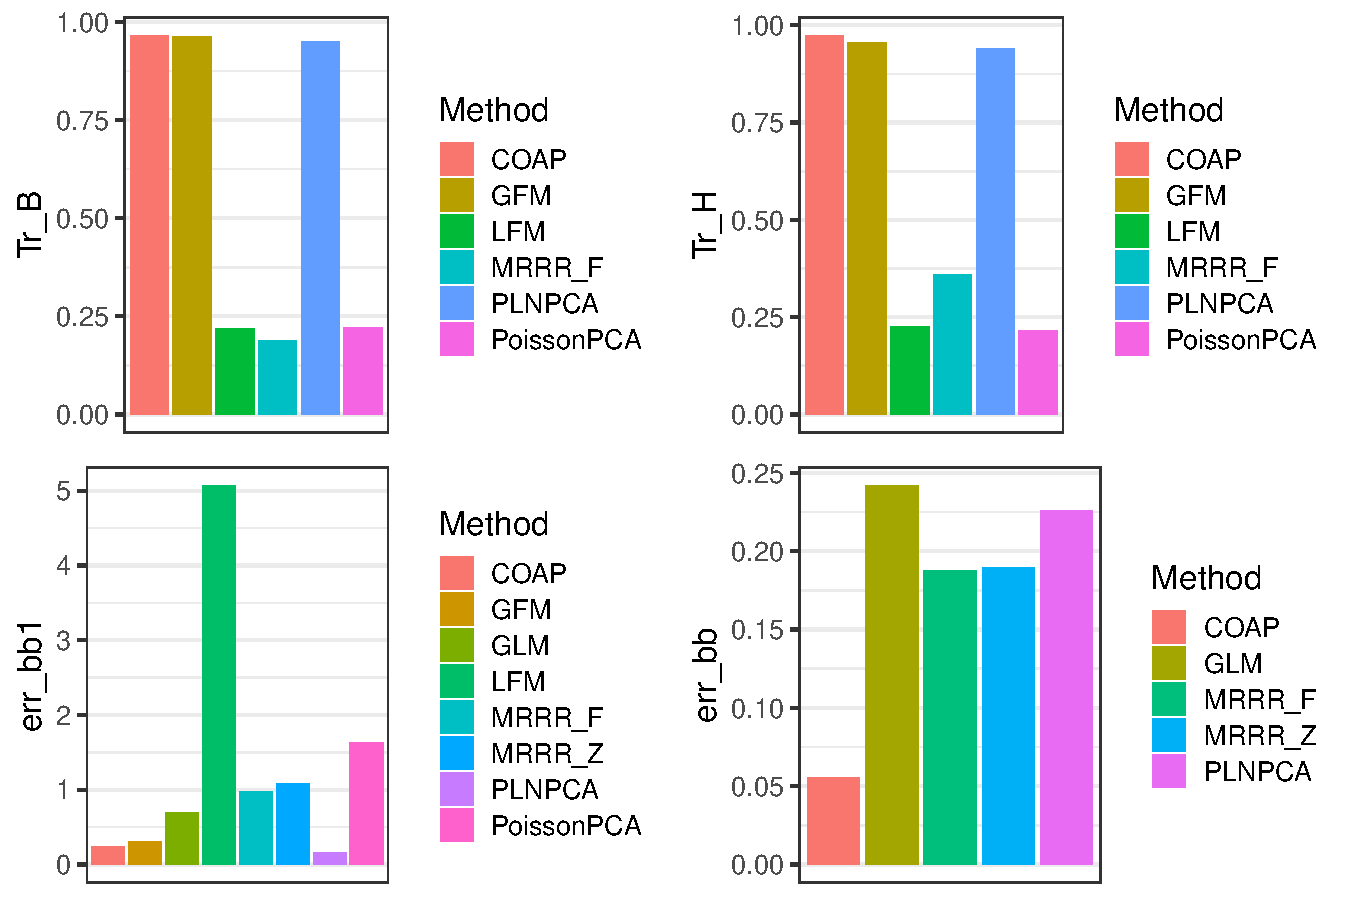
\includegraphics{COAPsimu_files/figure-latex/unnamed-chunk-17-1.pdf}

\hypertarget{select-the-parameters}{%
\subsection{Select the parameters}\label{select-the-parameters}}

We applied the singular value ratio based method to select the number of
factors and the rank of coefficient matrix. The results showed that the
SVR method has the potential to identify the true values.

\begin{Shaded}
\begin{Highlighting}[]

\NormalTok{datList <-}\StringTok{ }\KeywordTok{gendata_simu}\NormalTok{(}\DataTypeTok{seed =} \DecValTok{1}\NormalTok{,}\DataTypeTok{n=}\DecValTok{200}\NormalTok{, }\DataTypeTok{p=}\DecValTok{200}\NormalTok{, }\DataTypeTok{d=}\DecValTok{50}\NormalTok{, }\DataTypeTok{rank0 =} \DecValTok{6}\NormalTok{, }\DataTypeTok{q=}\DecValTok{5}\NormalTok{, }
                                       \DataTypeTok{rho=}\KeywordTok{c}\NormalTok{(}\DecValTok{3}\NormalTok{, }\DecValTok{6}\NormalTok{), }\DataTypeTok{sigma2_eps =} \DecValTok{2}\NormalTok{)}
\NormalTok{X_count <-}\StringTok{ }\NormalTok{datList}\OperatorTok{$}\NormalTok{X; Z <-}\StringTok{ }\NormalTok{datList}\OperatorTok{$}\NormalTok{Z}
\NormalTok{res1 <-}\StringTok{ }\KeywordTok{selectParams}\NormalTok{(}\DataTypeTok{X_count=}\NormalTok{datList}\OperatorTok{$}\NormalTok{X, }\DataTypeTok{Z=}\NormalTok{datList}\OperatorTok{$}\NormalTok{Z, }\DataTypeTok{r_max=}\DecValTok{20}\NormalTok{, }\DataTypeTok{verbose=}\NormalTok{F)}
\CommentTok{#> Calculate initial values...}

\KeywordTok{print}\NormalTok{(}\KeywordTok{c}\NormalTok{(}\DataTypeTok{q_true=}\NormalTok{q, }\DataTypeTok{q_est=}\NormalTok{res1[}\StringTok{'hq'}\NormalTok{]))}
\CommentTok{#>   q_true q_est.hq }
\CommentTok{#>        5        5}
\KeywordTok{print}\NormalTok{(}\KeywordTok{c}\NormalTok{(}\DataTypeTok{r_true=}\NormalTok{rank0, }\DataTypeTok{r_est=}\NormalTok{res1[}\StringTok{'hr'}\NormalTok{]))}
\CommentTok{#>   r_true r_est.hr }
\CommentTok{#>        6        6}
\end{Highlighting}
\end{Shaded}

\textbf{Session Info}

\begin{Shaded}
\begin{Highlighting}[]
\KeywordTok{sessionInfo}\NormalTok{()}
\CommentTok{#> R version 4.1.2 (2021-11-01)}
\CommentTok{#> Platform: x86_64-w64-mingw32/x64 (64-bit)}
\CommentTok{#> Running under: Windows 10 x64 (build 22621)}
\CommentTok{#> }
\CommentTok{#> Matrix products: default}
\CommentTok{#> }
\CommentTok{#> locale:}
\CommentTok{#> [1] LC_COLLATE=Chinese (Simplified)_China.936  LC_CTYPE=Chinese (Simplified)_China.936   }
\CommentTok{#> [3] LC_MONETARY=Chinese (Simplified)_China.936 LC_NUMERIC=C                              }
\CommentTok{#> [5] LC_TIME=Chinese (Simplified)_China.936    }
\CommentTok{#> }
\CommentTok{#> attached base packages:}
\CommentTok{#> [1] parallel  stats     graphics  grDevices utils     datasets  methods   base     }
\CommentTok{#> }
\CommentTok{#> other attached packages:}
\CommentTok{#>  [1] COAP_1.1         cowplot_1.1.1    rrpack_0.1-11    PLNmodels_1.0.1  PoissonPCA_1.0.3 ggplot2_3.4.1   }
\CommentTok{#>  [7] GFM_1.2.1        doSNOW_1.0.20    snow_0.4-4       iterators_1.0.14 foreach_1.5.2    irlba_2.3.5     }
\CommentTok{#> [13] Matrix_1.4-0     MASS_7.3-55      gllvm_1.4.1      mvabund_4.2.1    TMB_1.9.4       }
\CommentTok{#> }
\CommentTok{#> loaded via a namespace (and not attached):}
\CommentTok{#>  [1] sass_0.4.1            tidyr_1.2.0           jsonlite_1.8.0        bit64_4.0.5          }
\CommentTok{#>  [5] splines_4.1.2         bslib_0.3.1           assertthat_0.2.1      statmod_1.4.36       }
\CommentTok{#>  [9] highr_0.9             yaml_2.3.6            corrplot_0.92         globals_0.15.0       }
\CommentTok{#> [13] numDeriv_2016.8-1.1   pillar_1.9.0          lattice_0.20-45       glue_1.6.2           }
\CommentTok{#> [17] alabama_2022.4-1      torch_0.9.1           digest_0.6.29         colorspace_2.1-0     }
\CommentTok{#> [21] htmltools_0.5.2       pkgconfig_2.0.3       listenv_0.8.0         purrr_0.3.4          }
\CommentTok{#> [25] scales_1.2.1          processx_3.5.2        tibble_3.2.1          mgcv_1.8-39          }
\CommentTok{#> [29] farver_2.1.1          generics_0.1.2        withr_2.5.0           cli_3.2.0            }
\CommentTok{#> [33] survival_3.2-13       magrittr_2.0.3        evaluate_0.15         ps_1.6.0             }
\CommentTok{#> [37] future_1.26.1         fansi_1.0.4           parallelly_1.32.0     nlme_3.1-155         }
\CommentTok{#> [41] tools_4.1.2           lifecycle_1.0.3       stringr_1.4.0         lassoshooting_0.1.5-1}
\CommentTok{#> [45] glassoFast_1.0        munsell_0.5.0         glmnet_4.1-3          callr_3.7.0          }
\CommentTok{#> [49] packrat_0.7.0         jquerylib_0.1.4       compiler_4.1.2        tinytex_0.37         }
\CommentTok{#> [53] rlang_1.1.0           grid_4.1.2            nloptr_2.0.0          rstudioapi_0.13      }
\CommentTok{#> [57] tweedie_2.3.5         igraph_1.3.5          labeling_0.4.2        rmarkdown_2.11       }
\CommentTok{#> [61] gtable_0.3.3          codetools_0.2-18      DBI_1.1.2             R6_2.5.1             }
\CommentTok{#> [65] gridExtra_2.3         knitr_1.37            dplyr_1.0.9           fastmap_1.1.0        }
\CommentTok{#> [69] future.apply_1.9.0    bit_4.0.4             utf8_1.2.3            coro_1.0.3           }
\CommentTok{#> [73] shape_1.4.6           stringi_1.7.6         Rcpp_1.0.10           vctrs_0.6.1          }
\CommentTok{#> [77] tidyselect_1.1.2      xfun_0.29}
\end{Highlighting}
\end{Shaded}

\end{document}
